%Part of/Parte di https://github.com/f-dinucci/appuntiMeccanicaFluidi/
%License/Licenza Creative Commons Attribution-ShareAlike 4.0 International (CC BY-SA 4.0) - attribution/attribuzione Francesco Di Nucci
%See also/Vedere anche https://creativecommons.org/licenses/by-sa/4.0/ and/e https://creativecommons.org/licenses/by-sa/4.0/legalcode
%
\section{Fluido fermo e pressione}
\subsection{Fluido fermo e pressione}
Conviene semplificare i problemi visti finora con una riduzione delle incognite tramite simmetrie.

Una simmetria viene dalla definizione di fluido: un fluido è isotropo\footnote{da un punto di vista degli sforzi non vi sono sforzi tangenziali ed il modulo degli sforzi normali in un punto è costante}, quindi ha una simmetria di rotazione - le proprietà non cambiano in sistemi di riferimento ruotati tra loro a meno che non vi sia qualcosa che stabilisca una direzione privilegiata (cioè un vettore come $\uline{q}$).
Questo è legato ad un motivo fisico: mentre nei solidi le molecole sono incastrate in un reticolo, in un fluido sono libere di scorrere tra di loro in modo disordinato.
Nel caso speciale in cui il fluido sia fermo si ha che $\uline{q} = \rho \uline{v} = 0$, quindi non vi sono vettori che possano dare una direzione di riferimento.

Dato che non esistono vettori non nulli che abbiano componenti uguali in diversi sistemi di riferimento si ha che:
	\begin{equation*}
		\begin{aligned}
			\uline{J}_M = \uline{0} \\
			\uline{J}_E = \uline{0}
		\end{aligned}
	\end{equation*}
Ragionando su $J_{Qij}$, l'unico tensore rappresentato dalla stessa matrice in tutti i sistemi di riferimento è la matrice identità $\uuline{I}$ (o la matrice identità moltiplicata per un fattore costante $c$).
	\begin{equation*}
		J_{Qij} = c \delta_{ij} \quad \delta_{ij} = 
		\left\{ 
			\begin{aligned}
				1 \quad \text{se} \quad i=j \\ 
				0 \quad \text{se} \quad i \neq j 
			\end{aligned} 
		\right.
	\end{equation*}
La costante $c$ viene definita come pressione e indicata con la lettera $p$.

Si vedrà ora che ha le stesse proprietà della pressione come definita classicamente in fisica, analizzando il caso con un fluido statico della forza esercitata dal fluido sulla parete del contenitore. Si ha che:
	\begin{equation*}
		\uuline{J}_Q \vdot \uline{n} = p \uuline{I} \vdot \uline{n} = p \uline{n}
	\end{equation*} 
In caso di fluido a riposo si ha quindi che la forza $F$ esercitata su una generica superficie $S$ ha direzione normale alla superficie ed intensità $p$, coincidendo quindi con la definizione ``classica'' di pressione:
	\begin{equation*}
		\uline{F}_S = \int_S {\uuline{J}}_Q \vdot \uline{n} \dd{S} = \int_S p \uline{n} \dd{S}
	\end{equation*}

Inoltre, sempre nel caso di fluido fermo, il tensore flusso quantità di moto\footnote{che si vedrà coincidere con il tensore degli sforzi su una parete solida} si riduce al termine $pI$,  la pressione coincide quindi con la componente diagonale del tensore degli sforzi.
Nel caso di un fluido in movimento invece la forza esercitata sulla parete dipenderà oltre che dal contributo ``statico'' dovuto alla pressione, anche da altri termini dipendenti dalla velocità.

\subsubsection{Esempio di calcolo della pressione}
	\begin{figure}[h]
		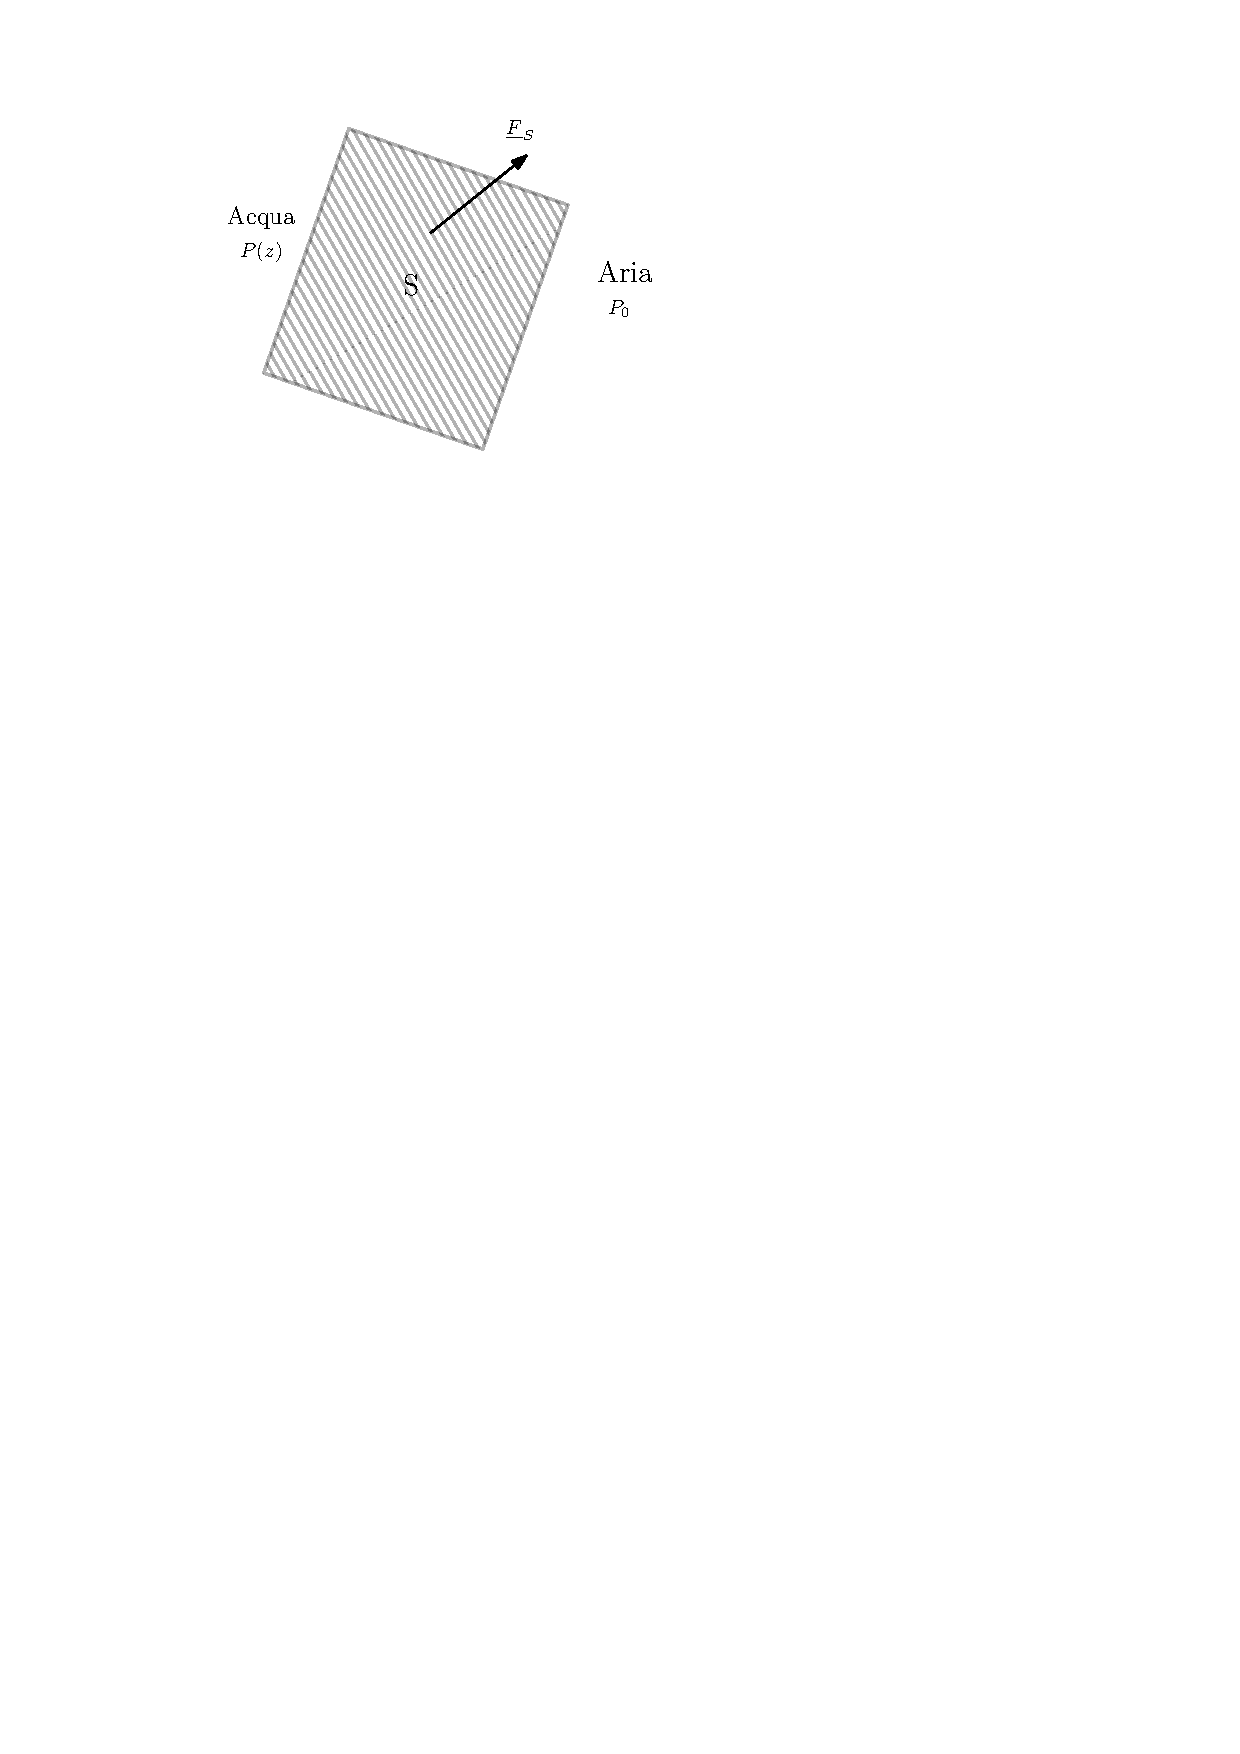
\includegraphics[scale=1.0]{./2.1 Fluido fermo e pressione/2.1-1}
		\centering
		\caption{Si prenda una superficie separante un volume d'acqua da uno di aria}
	\end{figure}
In questo caso si ha, considerando anche l'azione della pressione atmosferica, che:
	\begin{equation*}
		\uline{F}_S = \int_S (P - P_0) \uline{n} \dd{S} = \int_S \rho g (z - z_0) \uline{n} \dd{S}
	\end{equation*}

\subsection{Pressione assoluta e relativa}
Con pressione assoluta si intende il valore effettivo della pressione, che non può essere negativo.

Dato che in molti problemi, come in quello appena visto, conta la differenza tra questa e la pressione atmosferica più che la pressione assoluta, si introduce la pressione relativa\footnote{si sottintende relativa all'atmosfera}.
Questa è la differenza tra la pressione assoluta e quella atmosferica ($p_r = p - p_0$), e può essere negativa\footnote{in tal caso il suo valore assoluto è detto depressione}.
A seconda della pressione da misurare si utilizzano strumenti differenti: i manometri misurano pressioni relative, i vacuometri misurano pressioni assolute.
Sempre a seconda del contesto va considerata la pressione relativa od assoluta: nel caso di una automobile le gomme saranno sgonfie per una pressione uguale a quella atmosferica; per calcolare invece la forza agente sulla paratia di un razzo nello spazio occorrerà considerare la pressione assoluta (dato che oltre la paratia si trova il vuoto).

\subsection*{Bibliografia 2.1}
\cite[Cap.\ 3.1]{CengelCimbala}\\
\cite[Cap.\ 1.3.2]{LuchiniQuadrio}\\
\cite[Cap.\ 2.13]{PnueliGutfinger}



